% !TEX root = ../notes_template.tex
\chapter{Ventilation}\label{chp:alveolar_oxygen}
Updated on \today
\minitoc

Oxygen intake and carbon dioxide output are necessary for skeletal muscle energetics. The starting place of the intake of $O_2$ is drawing air into the lungs (ventilation) and the alveoli (alveolar ventilation). Similar, but opposite, the final expiration of $CO_2$ is releasing air out of the alveoli and lungs. This chapter covers alveolar ventilation ($V_A$), ventilation ($V_e$), ventilation/perfusion ($V/Q$) matching, the regulation of respiration through ventilation, and pulmonary insufficiency.  

\vspace{5mm}

\textbf{Objectives include:}
\begin{enumerate}
    \item Know and understand the material in the chapter.
    \item Connect and integrate material from other chapters with this chapter.
    \item Connect and integrate the material from this chapter with other chapters.
\end{enumerate}

\section{Ventilation Overview}

Chapter \ref{chp:blood_oxygen} on Respiration established the need for alveolar ventilation and alveolar circulation. There are three recurring and important preliminary concepts: alveolar ventilation ($V_A$), ventilation ($V_e$) and ventilation / perfusion matching ($V/Q$).

\subsection{Important Preliminary Concept}

\begin{itemize}
    \item Alveolar ventilation ($V_A$) is the movement of air into, and out of, the alveoli. Without continuous $V_A$ there is no alveolar respiration. 
    \item $V_e$ is the movement of air into, and out of, the lungs. $V_e$ is necessary for $V_A$. Without ventilation ($V_e$), there is no $V_A$. 
    \item Pulmonary perfusion is based on circulation ($Q$) and must be primarily distributed to alveoli receiving $V_A$. $V/Q$ matching refers to the matching of $V_A$ and pulmonary $Q$. Both $V_A$ and $Q$ are necessary for alveolar respiration. Without $V_A$ matching with pulmonary $Q$ there is no alveolar respiration.
 \end{itemize}

$V_e$ is the volume of air inspired (breathe in) or expired (breathe out) in a time period. It is most commonly measured in $mL/min$ or $L/min$. As a volume per minute, it is the volume of air per breath times the number of breaths per minute (bpm):
\vspace{3mm}
\begin{equation}
    V_e (mL/min) = V_t (mL) \times RR (bpm)
    \label{Ve}
\end{equation}
\vspace{3mm}

In Equation \ref{Ve}, the abbreviation $V_t$ stands for tidal volume. Tidal volume is the volume of air inspired (or expired) with one breath. The underlying assumption for both $V_e$ and $V_t$ is that the volume of air inspired equals the volume of air expired. While this might not be the case breath by breath, it tends to be the case over a minute (or longer) time periods.

\paragraph{Question:} What would happen if the volume inspired did not equal the volume expired over a long period of time? Try this, breathe more in than out, how long can you do that? Now breathe more out than in, how long can you do that?

\paragraph{} If there is an imbalance between $V_t$ in and $V_t$ out, it tends to be limited to transient periods that involve dynamic changes in $V_t$. For example, when $V_t$ increases in the transient periods from rest to exercise, or during exercise when there are variations in $O_2$ needs.

\paragraph{Not all $V_e$ ends in the alveoli ($V_A$)}, either per breath ($V_t$), or per minute ($V_e$). And, not all $V_A$ is going to be to alveoli with perfusion (receive capillary circulation). Figure \ref{fig:ve_va.jpg} depicts the general concept that $V_e$ is going to be greater than $V_A$; and that $V_A$ is going to be greater than the $V/Q$. Pulmonary regulation is largely based on minimizing the discrepancy between $V_e$, $V_A$ and $V/Q$.

\begin{figure}
    \centering
    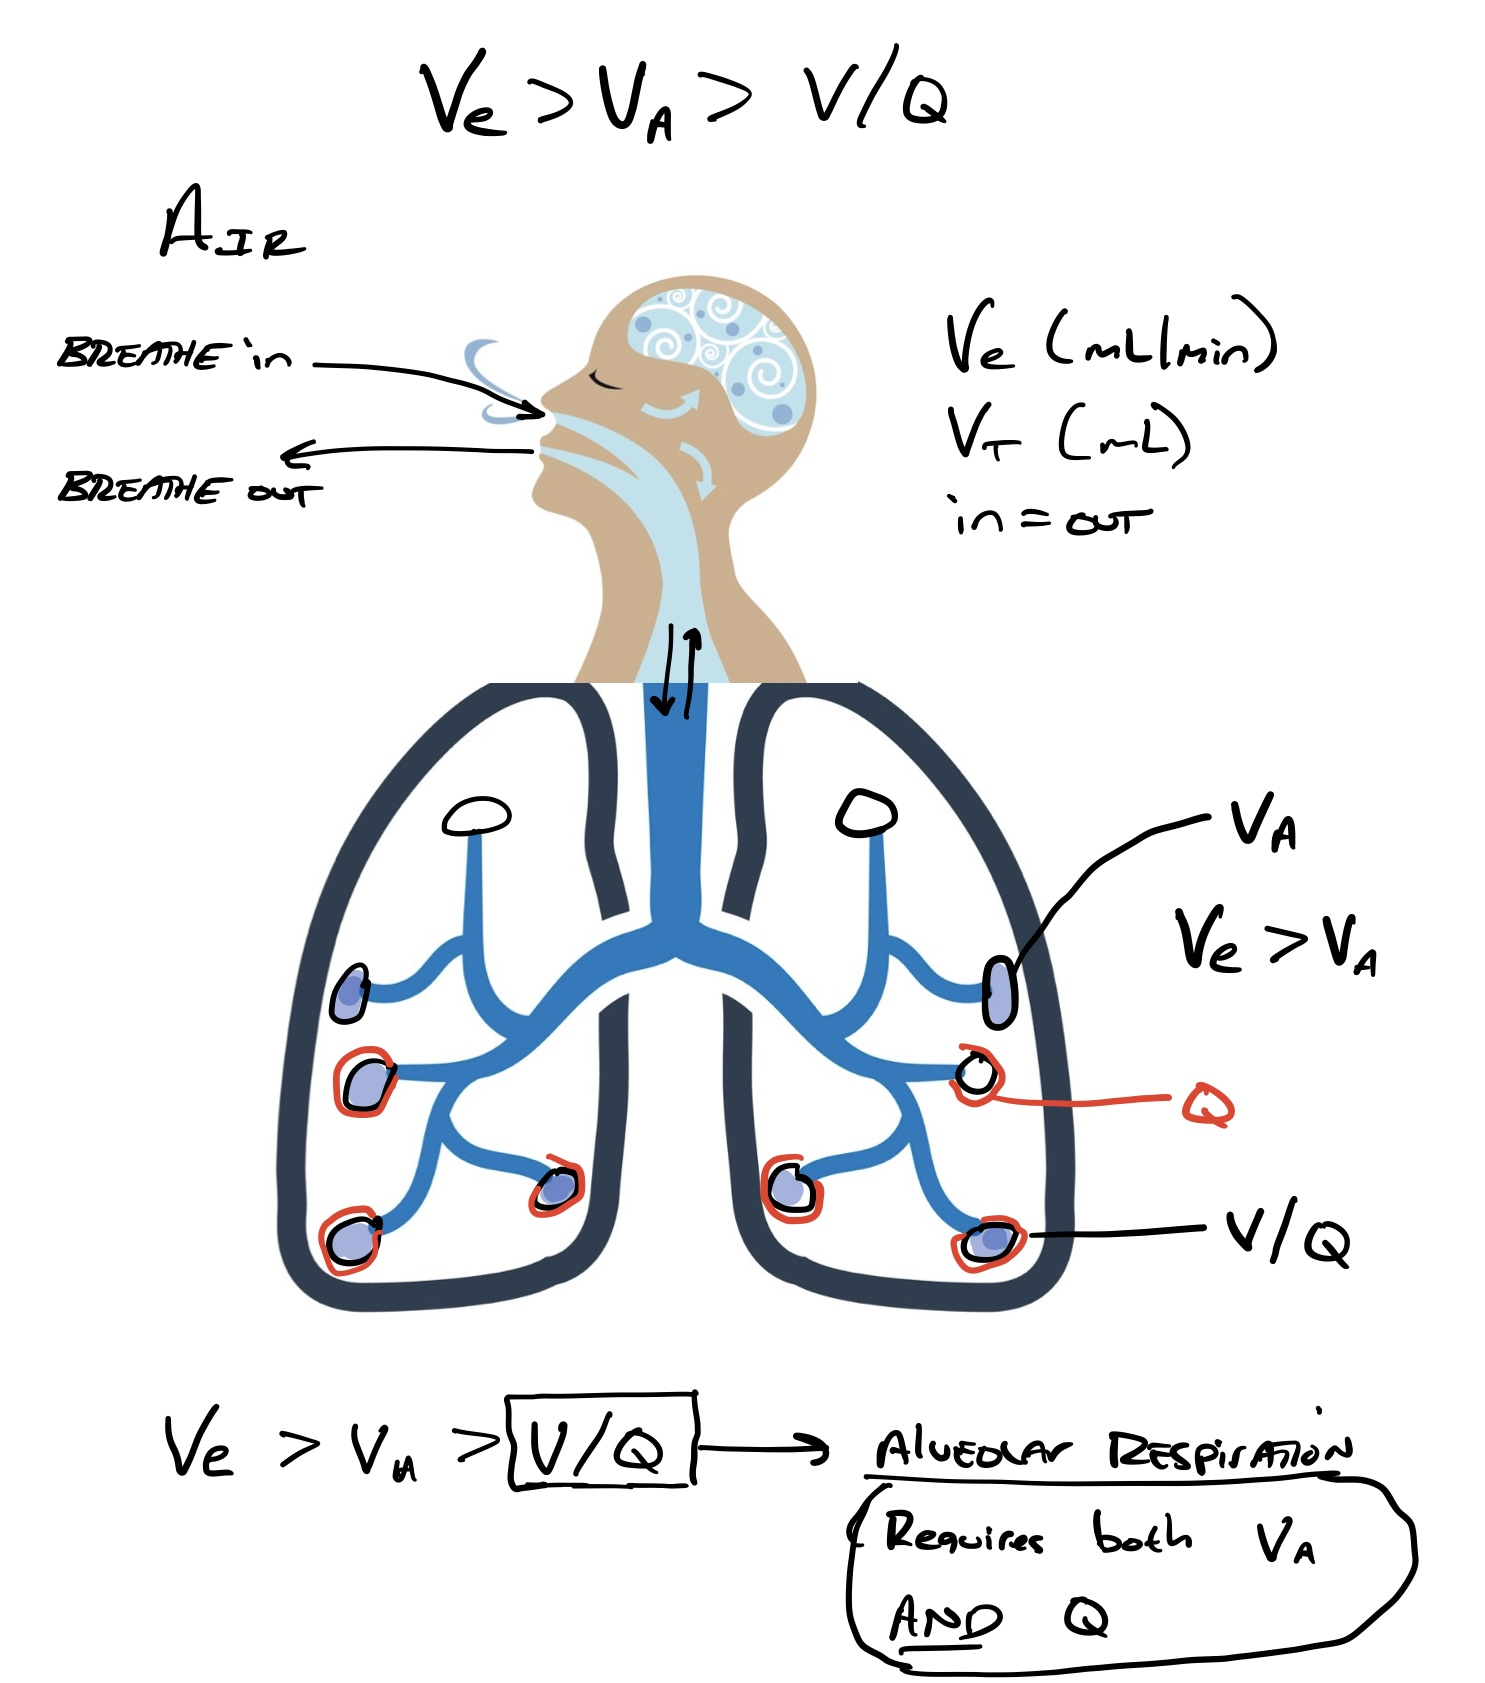
\includegraphics[width = 0.5\linewidth]{./figure/ve_va.jpg}
    \caption{Caption}
    \label{fig:ve_va.jpg}
\end{figure}

\paragraph{The importance of this concept} is that the alveolar respiration relies on the match between alveolar ventilation ($V_A$) and perfusion ($Q$). The consequences of all pulmonary (lung), and many cardiovascular, conditions ultimately rest on how they impact the ability to ventilate ($V_e$), the ability to turn as much $V_e$ into alveolar ventilation ($V_A$) as possible, or the ability to have as much $V_A$ perfusion as possible.

\subsection{Dead Space Ventilation ($V_D$}
Dead space ventilation that does not reach the alveoli (anatomical dead space), or that reaches the alveoli but does not receive perfusion (alveolar dead space). The combination of anatomical and alveolar dead space is called physiological dead space ($V_D$. To understand anatomical dead space ($VD_{ana}$) it is important to understand the structure and function of the airways.

\section{Airways}

The pathway of $O_2$ from the environment to the alveoli (or alveoli to the environment when considering $CO_2$) involves passage through a set of airways. It is important to recognize that only the alveoli are capable of gas exchange (diffusion, respiration). The difference between $V_e$ and $V_A$ starts with the airways.  

Figure \ref{fig:airways} includes the airways connecting the environment to the alveoli.

\begin{figure}[!h]
    \centering
    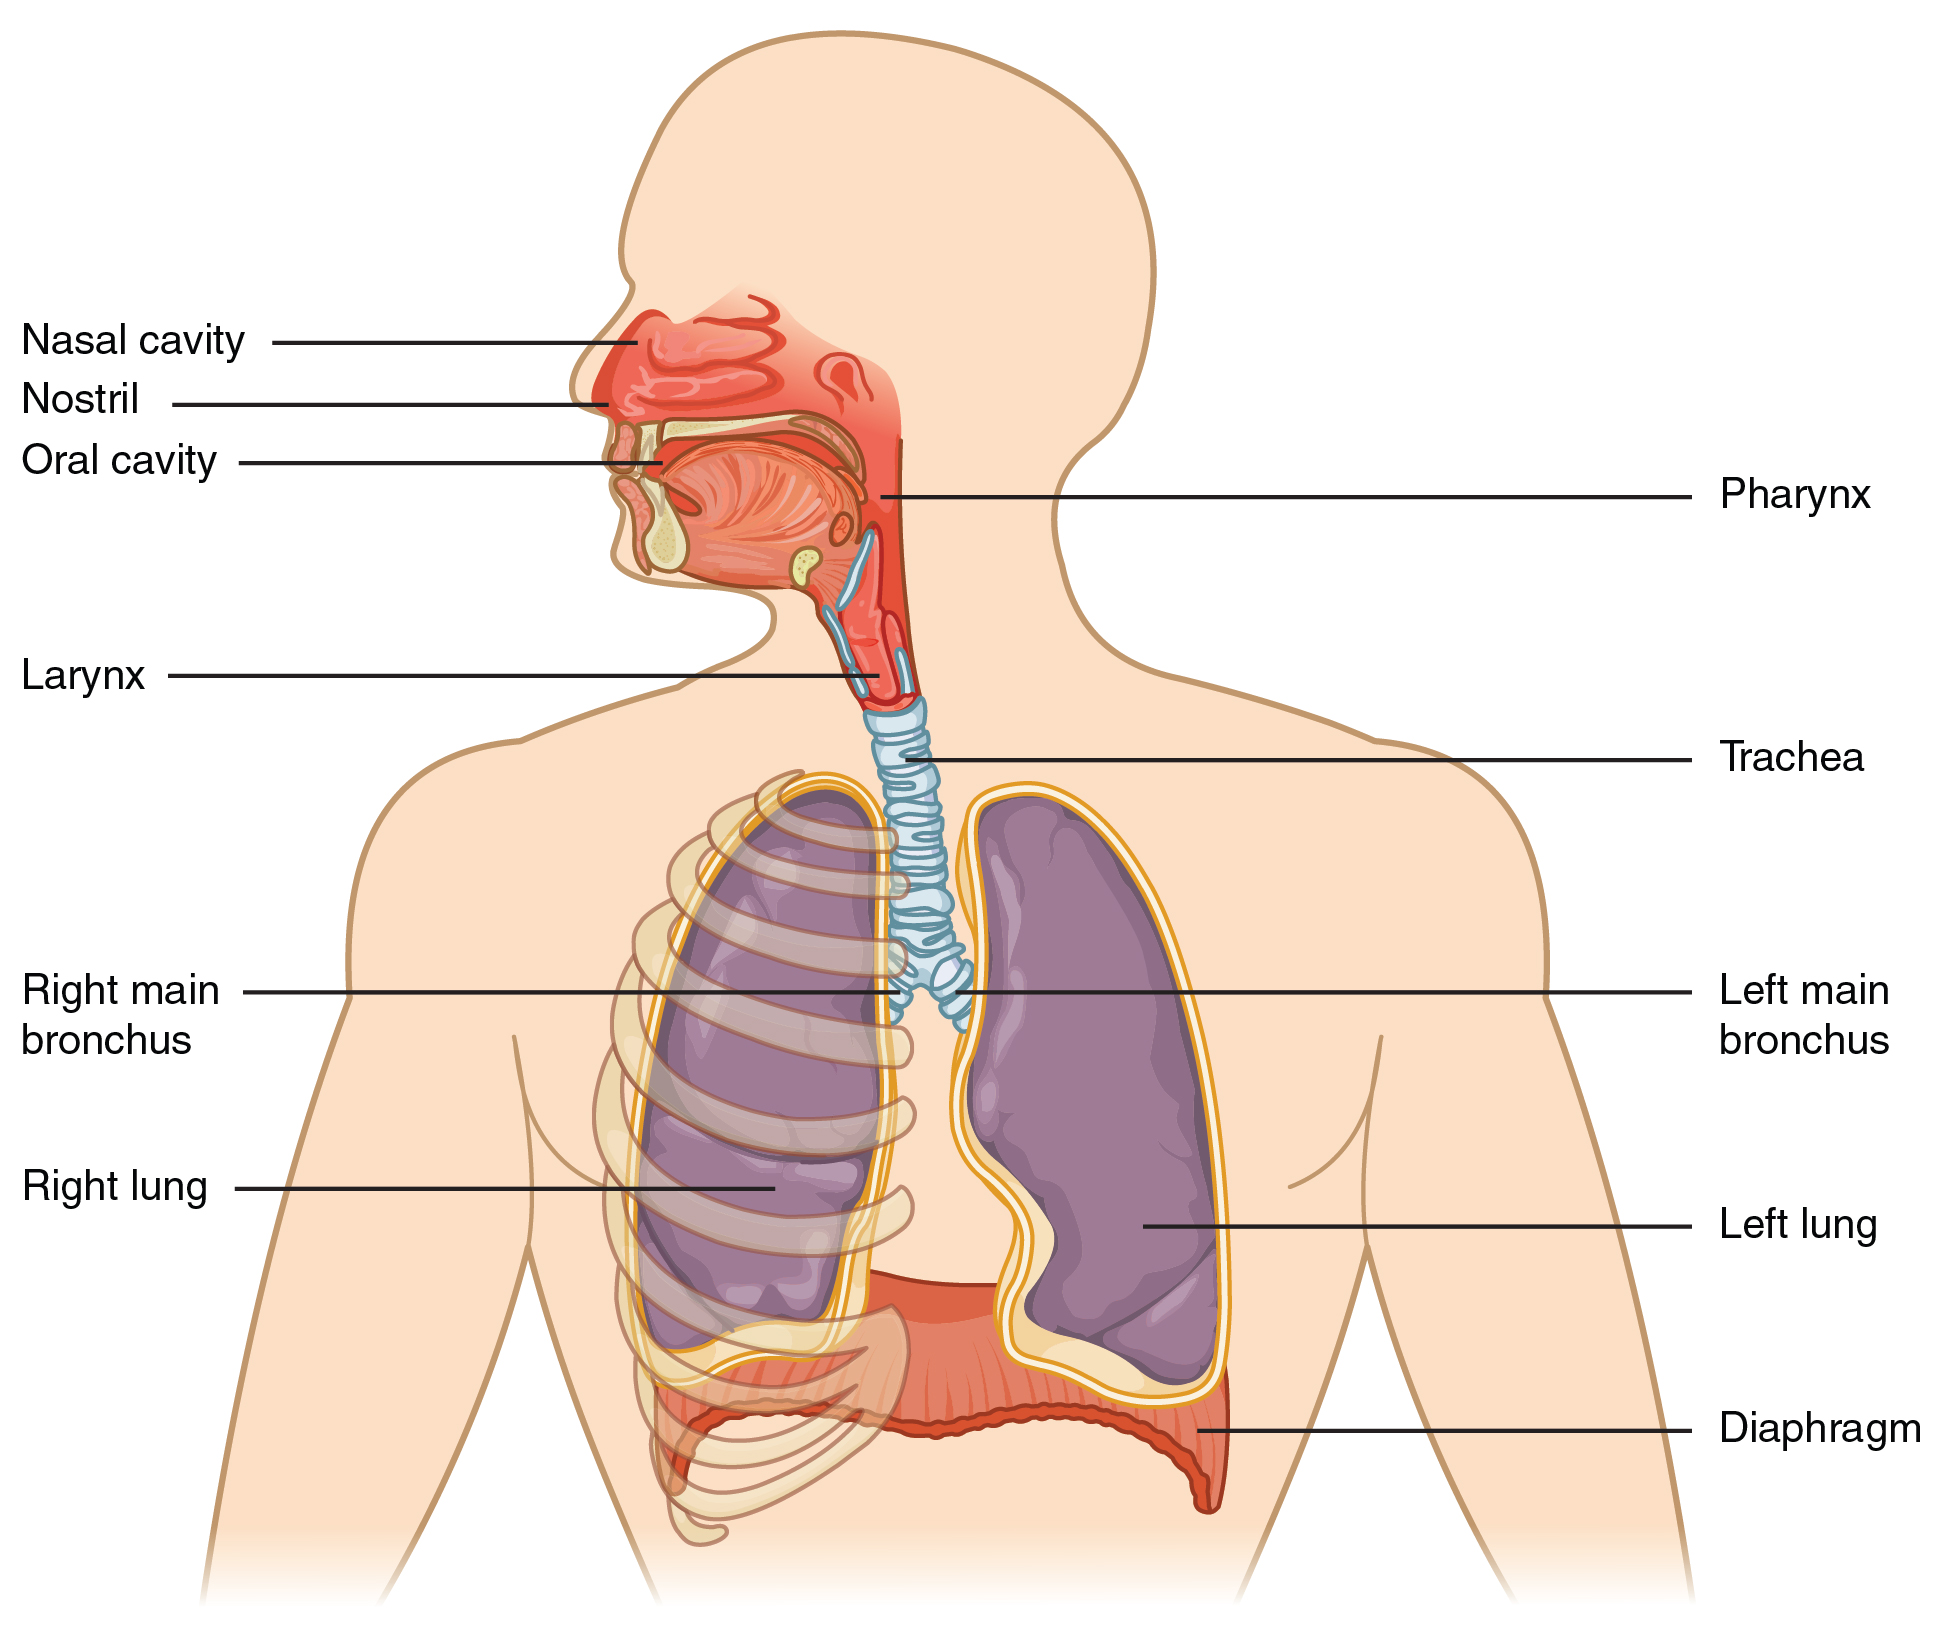
\includegraphics[width=1.0\linewidth]{./figure/airways.png}
    \caption{Passage to and from Alveoli}
    \label{fig:airways}
\end{figure}

\subsection{Anatomical Dead Space ($VD_{ana}$)}

Any air that enters the airways is part of $V_e$, but it is not part of $V_A$ unless it reaches an alveoli. For example, at the end of an inspiration the air remaining in the upper airways (nasal passages, the back of the throat, trachea) is part of $V_e$, but not part of $V_A$. The volume of air that is taken into the airways that does not reach the alveoli is referred to as anatomical dead space ($VD_{ana}$) and represents the conduction (non respiration) zone of the airways. $VD_{ana}$ is considered a fixed volume ($mL$). For example, if $VD_{ana} = 100 mL$, and 400 $mL$ is inspired with tidal volume ($V_T$), then 300 ($mL$) reaches alveoli ($V_A$). 

\paragraph{Question:}

Does $V_A (mL/min)$ change if $V_e (mL/min)$ stays the same but is achieved with different volume ($mL$) per breath at different breathing frequencies (respiratory rates)? Answer this by figuring out the $V_A (mL/min)$ and $V_e (mL/min)$ if $VD_{ana} = 100 mL$ when breathing 24 breaths per minute at 250 $mL/breath$; as compared to breathing 12 breathes per minutes at 500 $mL/breath$; as compared to breathing 6 breaths per minute at 1000 $mL/breath$. With each breathing pattern, $VD_{ana} = 100 mL$ since this is a fixed volume.

\subsection{Upper Airways}

The upper airways include the nasal passageways, the nasopharynx, the pharynx. Up to this point (the pharynx) the oral passages are also an option (but suboptimal) for breathing. The nasopharynx passes into the oropharynx which passes into the hypopharynx (laryngopharynx). At this point the epiglottis is the gatekeeper between the larynx (for air) and the esophagus (for food and drink).  The larynx includes the vocal cords and then continues into the trachea (beginning of the lower airways). 

All airway passages down as far as the terminal bronchioles are lined with epithelial cells that include, in various locations, mucus production cells and cilia. Cilia are small cellular extensions that promote the movement of substances such as mucus across the membrane surface. Cilia beat continually in a direction that moves mucus. The movement is toward the pharynx. Mucus and cilia in the airways are combined as a defense mechanism referred to as mucociliary activity. Together they promote the trapping of particles in mucus (including pathogens) and moving the mucus for removal. Cilia in the lower airways (trachea and bronchi) beat upward, whereas those in the upper airways beat downward. Continual beating moves the mucus toward the pharynx. The mucus and its trapped particles are then swallowed or coughed out of the body.

\subsubsection{Bronchopulmonary Hygiene \& Airway Clearance}
Mucocilary activity is an important component of what is called bronchopulmonary hygiene (BPH), while sneezing and coughing are called airway clearance. Techniques to facilitate airway clearance are airway clearance techniques (ACT). BPH and ACT include several manual techniques within the physical therapy scope of practice.\footnotemark\footnotetext{Please don't tell me that "respiratory therapy" does this, of course they do. But that does not negate the fact that this is part of the PT scope of practice. If PTs did not do the things in their scope of practice that other professionals do, physical therapists would not do anything. Saying "respiratory therapy" does this - is like saying "massage therapists" do this about soft tissue mobilization; or that "chiropractors" do this about joint mobs/manipulations; or that "athletic trainers" or "OTs" do this about rehabilitation; or that "exercise physiologists" or "personal trainers" or "strength and conditioning specialists" do this about exercise prescriptions. Of course that is all true. Doing one thing is NOT what makes any of those professionals the professionals that they are, it is doing those things in context and the variety of things being done that makes each of these professions, including physical therapy. The PT uses BPH-ACT in in the plan of care for patients receiving PT, which will undoubtably include many other interventions based on client needs.} Just as increasing tissue extensibility through manual techniques may facilitate the range of motion necessary to move during therapeutic exercise to then maintain tissue extensibility; improving ventilation and respiration through manual techniques may facilitate the respiration necessary to move during exercise to then maintain respiration.  

\subsubsection{Nasal Passageways} are lined with epithelial cells rich in olfactory sensors (sense of smell) and goblet cells which are responsible for creating the mucus membrane. The passages include a set of turbinates that create turbulent flow of air through the passageways which is important for immunity, humidification, adding nitric oxide and the sense of smell. The turbulent flow of air encourages interaction between the air entering the the nasal passages and the cellular epithelial mucus membrane. Large particles (dust, many pathogens, allergens) never move past becoming stuck in the mucus of the nasal passage membranes, serving an important immune and protective function. Interaction with the nasal passage membrane also humidifies the air (adds water) and adds nitric oxide (NO). NO enhances local defense mechanisms via direct inhibition of pathogen growth and stimulation of mucociliary activity. NO from the nose and sinuses is added to the air with every breath taken through the nose. NO reaches the alveoli in a more diluted form and enhances alveolar respiration by local vasodilation of pulmonary capillaries \cite{tornberg_nasal_2002, lundberg_nitric_2008}.

\subsubsection{Lower Airways}
The trachea is the airway that bridges the upper airways to the many airway divisions that will terminate in alveoli. The trachea is supported by cartilage rings that keep it open during wide fluctuations in thoracic pressures (coughing, sneezing, valsalva manuever). The trachea divides at the carina into two main bronchi (right and left) for the right and left lungs (respectively). 

The main, and larger bronchi, also contain cartilage rings for support along with smooth muscle. Each bronchi splits into two branches between 20-25 generations until ending with alveoli \cite{hall_guyton_2020}. The final branch of the bronchi is a bronchiole and is sometimes referred to as the respiratory bronchiole. The lower airways are also lined with epithelial cells that produce mucus and have cilia, and thus also have mucociliary activity that contributes to bronchopulmonary hygiene (BPH) and airway clearance. 

Similar to the artery to arteriole tree, each branch of the the bronchi to bronchiole tree gets progressively smaller, while the sum of space gets larger; and the influence of smooth muscle on the radius gets more important. For example, the main bronchi is larger than any single branch, but the branches, summed together, offer far more space than the main bronchi. As the branches get smaller with each generation of splitting the walls get thinner and the influence of smooth muscle on the walls gets more influential. Most bronchodilation and bronchoconstriction occurs in the smaller bronchioles than in the larger bronchi.

Under normal conditions resistance to air flow is highest in the larger bronchi because there are relatively few bronchi compared to bronchioles. But with various pulmonary conditions the smaller bronchioles can play a greater role in determining air flow resistance for two reasons. First, they are easily occluded because of their small size. Second, they are easily constricted because they have a greater proportion of smooth muscle fibers in their walls in relation to their radius.

The factors impacting air flow, like blood flow, through a cylinder such as an airway (or blood vessel) can be considered with Pouiselle's Law:
\vspace{3mm}
\begin{equation}
    Flow = \frac{\pi \times \Delta P \times r^4}{\eta \times L}
\end{equation}
\vspace{3mm}
And similar to blood flow, the resistance to airflow is largely determined, and manipulated, by changes to the radius through bronchodilation and bronchoconstriction.


\paragraph{Bronchodilation \& bronchoconstriction} are regulated by sympathetic nervous system innervation and endocrine function (circulating epinephrine and norepinephrine). Control of the bronchioles by sympathetic nerve fibers is relatively weak because few nerve fibers penetrate deeply and reach the bronchioles. However, all bronchi and bronchioles are exposed to circulating norepinephrine and epinephrine released from the adrenal gland medulla. These hormones, and in particular epinephrine because of its greater stimulation of β-adrenergic receptors, dilate bronchi and bronchioles. A few parasympathetic nerve fibers, from the vagus nerve, reach the bronchi and bronchioles. These nerves secrete acetylcholine, which constrict the bronchi and bronchioles. 
Conditions that create bronchoconstriction, such as asthma, are therefore commonly treated with adrenergic agonist inhalers (inhaled medication), sometimes in combination with cholinergic anatogonist inhalers or oral medications.  

\section{Volumes \& Capacities}

Ventilatory volumes and capacities are depicted in Figure \ref{fig:ventilation_volumes}. Capacities are combinations of volumes.

\begin{figure}[!h]
    \centering
    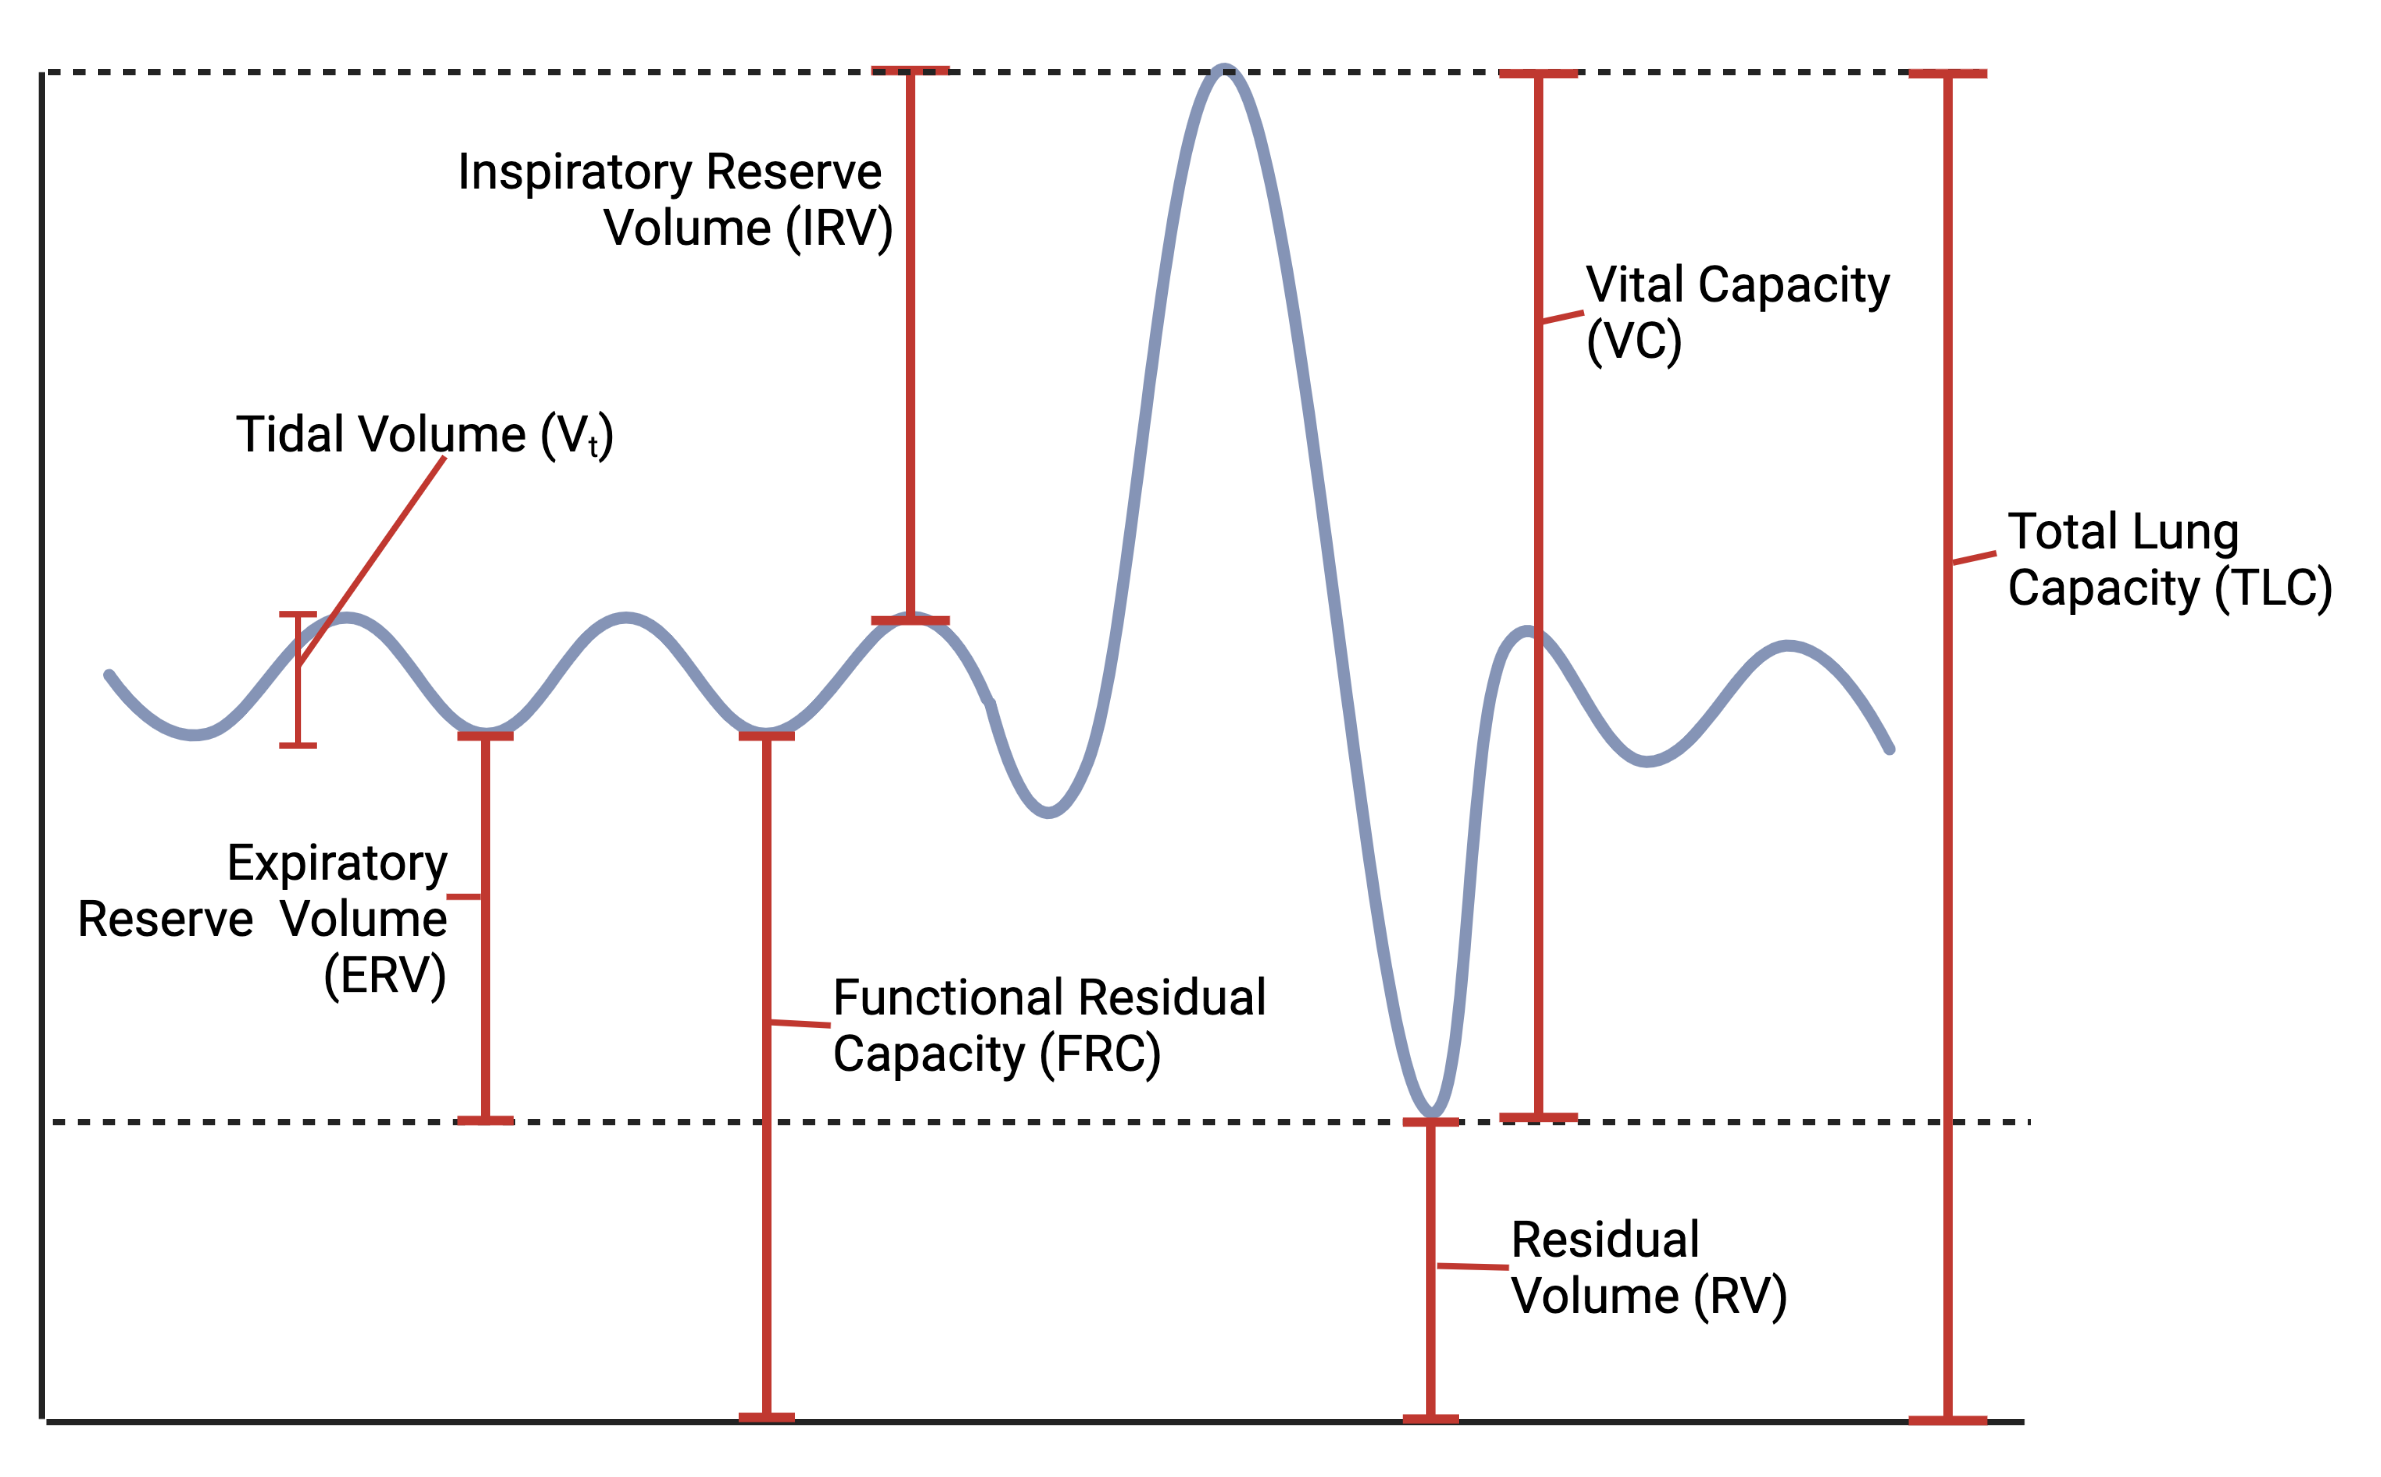
\includegraphics[width=1.0 \linewidth]{./figure/ventilation_volumes.png}
    \caption{Ventilatory Volumes \& Capacities}
    \label{fig:ventilation_volumes}
\end{figure}

\begin{itemize}
    \item Tidal Volume ($V_t$): Volume of breathing. $V_T$ varies in order to change ventilation $V_e$, for the purpose of changing $V_A$ to meet the needs of alveolar respiration as it maintains $Pa_CO_2$ and $P_aO_2$; or adjusts $Pa_CO_2$ as part of acid base balance regulation.
    \item Inspiratory Reserve Volume ($IRV$) is the volume that can be inhaled after a normal $V_t$ inspiration
    \item Expiratory Reserve Volume ($ERV$) is the volume that can be exhaled after the end of a normal $V_t$ expiration
    \item Residual Volume ($RV$) is the volume that cannot be exhaled
    \item Vital Capacity ($VC$) is $V_t + ERV + IRV$, it is the largest volume that can be breathed in after a complete exhalation, or out after a complete inspiration
    \item Functional Residual Capacity ($FRC$) is $ERV + RV$, it is the volume of air remaining in the lungs after a normal expiration
    \item Total Lung Capacity ($TLC$) is $IRV + V_t + ERV + RV$, it total capacity for air in the lungs
\end{itemize}

\paragraph{The Musculoskeletal Side of Ventilation} Volumes \& capacities are measures the amount of air that can be ventilated (or that cannot be ventilated in the case of $RV$ which cannot be expired). They are used to better understand the functional capabilities of the lungs and describe changes to the lung in various states of disease. For example, with the obstructive pulmonary diseases the $RV$ tends to be higher, which reduces $VC$ (and all other values, except $FRC$). However, the volumes \& capacities also represent a functional measure of the thoracic cavity musculoskeletal range of motion (chest wall mobility) which includes the diaphragm, muscles of the ribs (intercostal muscles), the mobility of the ribs, and the posture of the spine. For example, in situations with diaphragm weakness, reductions in $VC$ are directly related to an inability of the diaphragm to fully descend against the combined resistance pulmonary elasticity and abdominal contents. In patients with many different neurological conditions there is involvement of ventilatory muscles or spinal posture which greatly influence the ventilatory volume \& capacities that further limit activities and result in pulmonary conditions such as pneumonia.

\paragraph{Volumes \& Capacities as ROM or Position:} Occasionally the volumes and capacities are utilized as an indication of the chest wall ROM or position in a very general way. During testing of the strength of inspiratory muscles patients are asked to expire all their air prior to the test because it is best to test those muscles when they are stretched. Those muscles are stretched when they are in the position of, at the ROM of, $RV$. When doing a forced expiration, or when training someone to improve their cough, they are asked to take in a full breath, they breath in until $TLC$ or $VC$. 

\paragraph{} Physical therapists contribute uniquely to problems related to breathing and ventilation because of how much these processes rely on the neuromuscular mechanics of the breathing muscles. Like posture, gait and many movements, the breathing muscles and patterns of ventilation are mostly automatic yet are able to be voluntarily controlled, and therefore manipulated, adapted and trained.

\subsection{Mechanics: The Ventilatory Pump}

The ventilatory pump that creates the pressure for ventilation involves the musculoskeletal system of the thorax (chest wall), including the diaphragm as the floor of the thoracic cavity (and roof of the abdominal cavity, See Figure \ref{fig:diaphragm_lateral}). The diaphragm is positioned to contribute to the variation of pressures between the thoracic and abdominal cavities which makes it uniquely involved in breathing as well as the coordination of breathing with other aspects of dynamic core stability. 

\begin{figure}[!h]
    \centering
    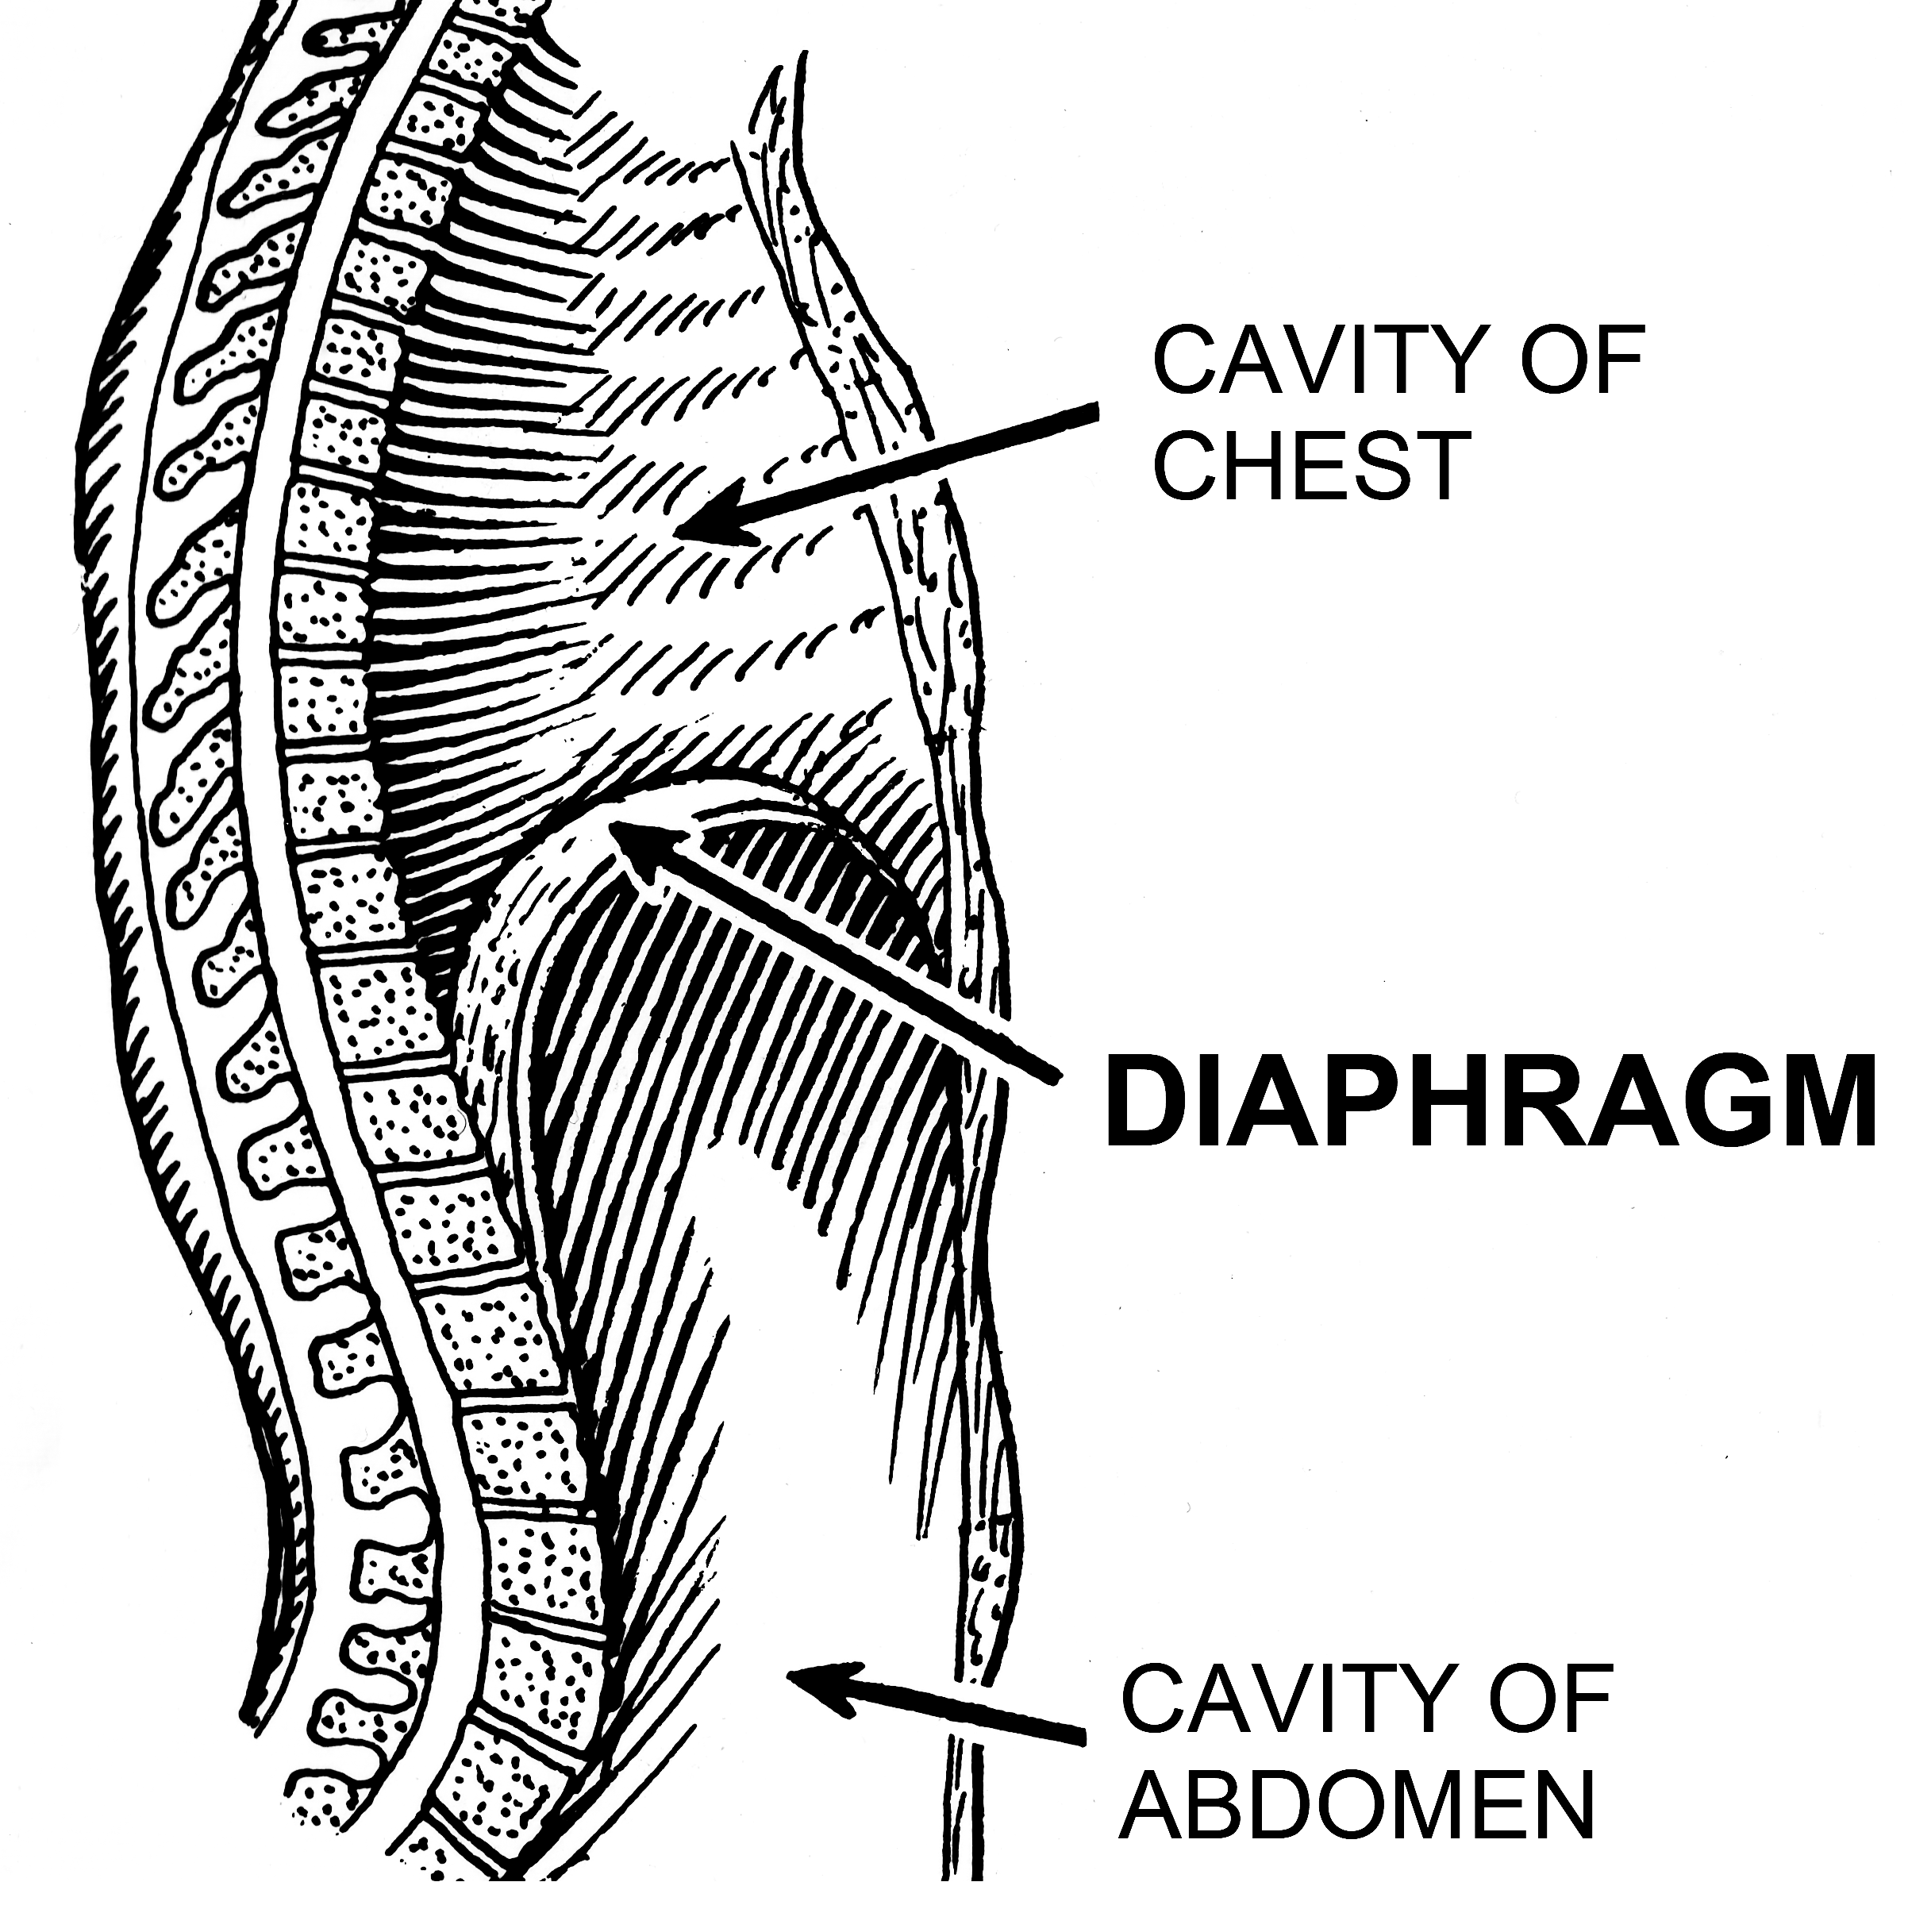
\includegraphics[width=0.5 \linewidth]{./figure/diaphragm_lateral.png}
    \caption{Caption}
    \label{fig:diaphragm_lateral}
\end{figure}

\paragraph{Inspiration: A Negative Pressure Pump} For breathing air into the lungs the ventilatory pump is a negative pressure pump. Rather than generating positive pressure that pushes air into the lungs, it generates negative pressure that pulls air into the lungs. It does this by expanding the volume of the thoracic cavity, which lowers the pressure below the atmospheric pressure to establish the necessary pressure gradient for air flow. Based on the now, hopefully, familiar equation: $Flow = (P_1 - P_2) / R$; the flow is directly proportional to the pressure gradient created, and inversely proportional to the resistance (and the resistance is largely dependent on the radius of the airways). 

\paragraph{Expiration: A Positive Pressure Pump} For breathing air out of the lungs the ventilatory pump is a positive pressure pump. Positive pressure is generated by contracting the volume of the thoracic cavity, which increases the pressure above the atmospheric pressure to establish the necessary pressure gradient for air flow. Air flow is still directly proportional to the pressure gradient, and inversely proportional to resistance. Resistance is still largely dependent on the radius of the airways. 
One difference with expiration is that the positive pressure, combined with the fact that during expiration the lungs and airways are getting smaller, it is much more likely that resistance to expiratory flow will impact exhalation (than resistance to inspiratory flow will impact inhalation). The practical implications are that with any condition that impacts airway radius, such as asthma, emphysema and chronic bronchitis, the functional impact is on expiratory flow rates more so than inspiratory flow rates. When a limitation is made on expiratory flow rates the term utilized to describe the pattern is obstructive. 
Forced expiratory activities - such as airway clearance with sneezing or coughing - requires a rapid increase in positive thoracic pressure. The difference between a sneeze (besides being typically through the nose) and a cough is closure of the epiglottis to allow for a larger build up of positive pressure in the thoracic cavity and a sudden release of that pressure when the epiglottis opens.  

\paragraph{Pressure Equilibration} Airflow through airways is rapid enough that equilibration can occur at any thoracic cavity volume. Once equilibration occurs, airflow stops. This means that at any thoracic cavity volume, other than $TLC$ or $RV$, changes in volume can cause either inspiration or expiration depending on how the changes in volume change the pressure. At this point it's helpful to remind readers of the Ideal Gas Law (in fact, this needs to be introduced earlier to avoid confusion in future versions....). 

The common form of the Ideal Gas Law is: 

\begin{equation}
    PV = nRT
    \label{ideal_gas}
\end{equation}

Where, $P$ is pressure; $V$ is volume, $n$ is the number of moles in the gas (the amount of gas), $R$ is a gas constant, and $T$ is the temperature in Kelvin. For our purposes we can simplify by removing $R$ and $T$ (although there are slight changes during ventilation from the temperature of atmospheric air and the warmed air at body temperature, these are relatively small on the Kelvin scale, and since we are not actually calculating just considering relationships, we'll be fine).

A simplified version of the Ideal Gas Law, that solves for $P$ is:

\begin{equation}
    P = \frac{n}{V}
\end{equation}

An increase in the thoracic cavity $V$ will reduce the $P$, but air will flow into the thorax through airways until the amount of air in the lungs $n$ equilibrates the equation so that $P$ really does equal $\frac{n}{V}$. Once $P$ in the lungs equals the atmospheric $P$, airflow stops. At that point, if thoracic cavity $V$ can be increased more then $P$ will drop and more air will flow into the lungs until $n$ increases to the point that the equation is once again balanced (equilibrated). This occurs until $P$ in the lungs equals atmospheric $P$. 
The same process can be considered for exhalation. A reduction in thoracic cavity $V$ increases the $P$, air flows out of the lungs until $n$ is reduced to the point of the equation being balanced and the lung $P$ equals the atmospheric $P$. 

\paragraph{Breathing in, Breathing out} is a cyclic variation in the difference between the thoracic (pulmonary) $P$ and the atmospheric $P$, brought on by the cyclic variation in the thoracic (pulmonary) $V$, which is equilibrated by the movement of air into (increase $n$) and out of (decrease $n$) the lungs.

\subsubsection{$FRC$: The Resting Position}

When considering the mechanics of the ventilatory pump during breathing it is useful to understand the conditions surrounding the functional residual capacity ($FRC$). $FRC$ is the resting position (volume) of the thoracic cavity, and therefore the amount of air in the lungs at this position equals the $FRC$. (That's a nice, intentionally, circular explanation.) 
More importantly, $FRC$ is the $V$ of the thoracic cavity when there is no active tension being developed by the breathing muscles. The $V$ of the thoracic cavity can still change based on body position, but it is not changing due to active tension of breathing muscles (either inspiratory or expiratory muscles). If you "stop breathing" - and there is no airflow - you are at $FRC$. If you do this in standing and then sit down there may be slightly less $V$ at $FRC$. If you are seated upright and slouch or lean forward then you reduce the $V$ and $FRC$. 

\paragraph{$FRC$ is the balance point} between an inward elastic recoil force of the lung tissue, and an outward elastic recoil force of the musculoskeletal thoracic cavity. If the lungs were removed from the body, they would be smaller (less $V$) than at the $FRC$. The thoracic cavity would be larger (more $V$) than at the $FRC$. During resting tidal volume ($V_t$) breathing each expiration ends at $FRC$ and therefore is a passive process. Each inspiration requires muscles of inspiration to expand the thoracic cavity $V$, working against the passive recoil force of the lung tissue. But then the passive recoil force of the lung returns the $V$ to $FRC$ which promotes expiration. Therefore, with resting $V_t$ breathing only the muscles of inspiration must be utilized. 
During resting $V_t$ breathing early increases in thoracic cavity $V$ are easier to perform because the thoracic cavity is naturally larger than at $FRC$. However, with increases in thoracic cavity $V$ both the lungs and the thoracic cavity create a passive elastic force that the muscles of inspiration must oppose for continued inspiration. This is one of the reasons why during exercise, breathing patterns typically increase $V_t$ by using more of the $ERV$ as compared to the $IRV$.

Forceful expiration requires a larger and more rapid change in $P$, which requires a larger and more rapid change in $V$, which requires active tension in the muscles of expiration. Increasing the rate of breathing $RR$ alone, or along with an increase in $V_t$, requires active tension of the expiratory muscles so that it occurs more completely (volumes less than $FRC$), and more quickly. 

\subsubsection{Muscles of Inspiration: Increase Thoracic Cavity Volume}

\paragraph{Diaphragm}

The diaphragm is a membranous muscle and is the most important inspiratory muscle, with motor innervation solely from the phrenic nerves (C3-C5). The diaphragm is extremely active. Muscle fibres within the diaphragm can reduce their length by up to 40\% between residual volume and total lung capacity and spend 35\% of each day contracting, compared with only 14\% for the soleus muscle (Cite Nunn). The origins of the crural part of the diaphragm are the lumbar vertebrae and the arcuate ligaments, while the costal parts arise from the lower ribs and xiphisternum. Both parts are inserted into the central tendon. 
Under normal circumstances, a zone of apposition exists around the outside of the diaphragm where it is in direct contact with the inside of the rib cage, with no lung in between. The parietal pleura continues to allow movement of the diaphragm. When at the upright $FRC$ approximately 55\% of the diaphragm surface area is in the zone of apposition.

There are three primary ways that the diaphragm creates increased thoracic cavity $V$ and these three ways are combined during breathing. Diaphragm mechanics can be considered with the analogy to a piston in a cylinder. With the diaphragm being the piston, and the thoracic cavity being the cylinder. 

\begin{enumerate}
    \item Piston: Downward movement of the diaphragm simply by shortening the zone of apposition around the whole cylinder and leaving the dome shape unchanged. This action very efficiently converts diaphragm muscle shortening into changes in $V$.
    \item Non Piston: Diaphragm tension reduces the curvature and therefore the dome shape. This does not change the zone of apposition but results in an, albeit smaller, increases the $V$.
    \item Piston in an Expanding Cylinder: The diaphragm pulls upward on the lower rib cage resulting in expansion of the lower thorax and therefore thoracic cavity $V$. This contributes to the "bucket handle" movement of the lower rib cage during breathing.
\end{enumerate}

There are many factors that influence how the above three ways that diaphragm mechanics contribute to inspiration. What is clear is that the larger the inspiratory volume, the more diaphragm activity is required and the likelihood that all three mechanical approaches are involved. The two most important factors influencing these mechanics are activity (which influences the amount of air that must be ventilated ($V_e$)); and the posture. For example, in supine the "Piston in an Expanding Cylinder" approach tends to dominate because abdominal mass reduces downward movement of the diaphragm which increases upward pull on the lower ribs.

\paragraph{Intercostals \& Scalenes}

The exact coordination and involvement of the external and internal intercostals during breathing is complicated and most descriptions (including this one) is a simplification. There are several contradictory sources about which set of intercostals are involved with inspiration vs. expiration. To avoid those contradictions, and since there is little practical value to those arguments, we simply consider the intercostals and do not attempt to assign a particular breathing role to the external or internal sets. We rather consider both the internal and external as contributing to either lifting the ribs (for inspiration) or lowering the ribs (for expiration) from their axes at the costotransverse and costovertebral joints in the thoracic spine. We consider this based on motor coordination patterns.

The inspiration motor coordination pattern for the intercostals starts with the activation of the scalenes. Scalenes are active even during quiet breathing. They stabilize the first rib. The first rib is then the anchor for each rib below it, in succession, to pull upward on the rib below it. They support, or pull up, rib 1. From this base of support the intercostals between rib 1 and 2 stabilize, or pull up, rib 2. From the base of support at rib 2, the intercostals between rib 2 and 4 stabilize, or pull up, rib 3. The pattern continues to rib 12 - the stabilized rib n, allows the intercostals between rib n and n+1 to stabilize, or pull up, rib n+1.

Based on the costotransverse and costovertebral joint axes, and in combination with attachment to the sternum, the upward movement of the upper ribs (1 - 6 or so), is described as "pump handle" which includes a change in the anteriorposterior (AP) diameter of the thoracic cavity. The upward movement of the lower ribs (7ish through 12) is described as "bucket handle" which includes a change in the medial-lateral (ML) diameter of the thoracic cavity.

Even during quiet breathing there is active tension generated in the scalenes and intercostals, even if there is no movement of the ribs. These isometric contributions at the very minimum, prevent inward movement of the ribs due to the drop in thoracic pressure by the piston action of the diaphragm. In premature infants with underdeveloped intercostal muscles, or people with C5 to C8 spinal cord injury that do not have innervation of the intercostal muscles, a thoracic paradox breathing pattern can impair ventilation. This breathing pattern includes a diaphragm piston like activation that reduces thoracic pressure and pulls the ribs inward which reduces the change in thoracic $V$ and limits ventilation. It is thoracic paradox because the thoracic is not doing what is expected during inspiration. Can you figure out what an abdominal paradox breathing pattern is and when it might occur?

\paragraph{Accessory Inspiratory Muscles}
Accessory muscles are not active during normal breathing, but as ventilation increases and the inspiratory muscles contract more vigorously accessory muscles are recruited. Other reasons for accessory muscle activation may be when there are limitations in the primary muscles or when there are pulmonary conditions making ventilation less efficient. Accessory muscles include the sternocleomastoids, extensors of the vertebral column, pectoralis minor (and to a lesser extent major), trapezius and the serratus anterior and posterior muscles. For many of these muscles to serve an accessory role to inspiration the upper extremity must be stabilized so that tension in the muscle moves the thorax, not the limbs. In people with severe pulmonary disease that rely on accessory muscle activation for breathing, activities that use the upper extremities can be considerably limited.

% Left off here....

\subsubsection{Muscles of Expiration: Decrease Thoracic Cavity Volume}

\paragraph{Intercostals}

\paragraph{Abdominal Muscles}

\paragraph{Accessory Expiratory Muscles}


During heavy breathing, the elastic forces are not sufficiently powerful to cause rapid expiration. The extra force is achieved mainly through contraction of the abdominal muscles, which pushes the abdominal contents upward against the diaphragm. Raising and Lowering the Rib Cage Causes the Lungs to Expand and Contract When the rib cage is elevated, the ribs project almost directly forward, so the sternum also moves forward and away from the spine, increasing the anteroposterior thickness of the chest. • Muscles that raise the rib cage are muscles of inspiration. Contraction of the external intercostals causes the ribs to move upward and forward in a “bucket handle” motion. Accessory muscles include the sternocleidomastoid muscles, the anterior serrati, and the scaleni. • Muscles that depress the rib cage are muscles of expiration, including the internal intercostals and the abdominal recti. Other abdominal muscles compress the abdominal contents upward toward the diaphragm.

Pressures That Cause Movement of Air in and out of the Lungs (p. 491) Pleural Pressure Is the Pressure of the Fluid in the Space Between the Lung Pleura and Chest Wall Pleura The normal pleural pressure at the beginning of inspiration is about −5 cm of water (cm H2O), which is the amount of suction required to hold the lungs at their resting volume. During inspiration, expansion of the chest cage pulls the surface of the lungs with greater force and creates a more negative pressure, averaging about −7.5 cm H2O. Alveolar Pressure Is the Air Pressure Inside the Lung Alveoli When the glottis is open and there is no movement of air, the pressures in all parts of the respiratory tree are equal to atmospheric pressure, which is considered to be 0 cm H2O. • During inspiration, pressure in the alveoli decreases to about −1 cm H2O, which is sufficient to move about 0.5 L of air into the lungs within the 2 seconds required for inspiration. • During expiration, opposite changes occur. The alveolar pressure rises to about +1 cm H2O, which forces the 0.5 L of inspired air out of the lungs during the 2 to 3 seconds of expiration. Lung Compliance Is the Change in Lung Volume for Each Unit of Change in Transpulmonary Pressure Transpulmonary pressure is the difference between the alveolar and pleural pressures. The normal total compliance of both lungs together in the average adult is about 200 ml/cm H2O. Compliance depends on the following forces: • Elastic forces of the lung tissues are determined mainly by the elastin and collagen fibers. • Elastic forces caused by surface tension in the alveoli account for about two-thirds of the total elastic forces in normal lungs. Surfactant, Surface Tension, and Collapse of the Alveoli (p. 493) Attraction of Water Molecules to One Another Exerts Surface Tension Elastic Force The watery surface lining the alveoli attempts to contract because the water molecules pull toward one another. This force attempts to move air out of the alveoli, causing the alveoli to attempt to collapse. The net effect is to cause an elastic contractile force of the entire lung, called the surface tension elastic force. Surfactant Reduces the Work of Breathing (Increases Lung Compliance) by Decreasing Alveolar Surface Tension Surfactant is secreted by type II alveolar epithelial cells. Its most important components are phospholipid dipalmitoyl phosphatidylcholine, surfactant apoproteins, and calcium ion. The presence of surfactant on the alveolar surface reduces the surface tension to one-twelfth to one-half of the surface tension of a pure water surface.



Inspiratory muscles - primarily diaphragm (phrenic nerve, C1-3); diaphragm tensions pulls the thoracic cavity down (central tendon extends down to it's attachments); and it pulls up on the lower ribs


internal intercostals, any muscle that can expand the chest wall (spinal extensors, scalenes, sternocleomastoid)

Expiratory muscles - only needed during exhalation at rates greater than resting tidal breathing, or forced expiratory manuevers such as sneezing, coughing; external intercostals; abdominal muscles (including transverse abdominus, internal and external obliques, rectus abdominus)

Rib movements


\subsection{Pressures}





\section{Ventilation - Perfusion Matching}

\begin{itemize}
       \item Anatomical dead space is air ventilated but that does not make it into alveoli. Anatomical dead space = $V_e - V_A$
    \item Physiological dead space occurs in alveoli that receive ventilation but do not receive alveolar circulation
    \item Dead space ventilation ($V_{DS}$) is the sum of anatomical and physiological dead space
\end{itemize}


Chapter \ref{chp:alveolar_oxygen} on Ventilation considers the concept of ventilation - perfusion $\dot{V}/\dot{Q}$ matching, the impact of body position on $\dot{V}/\dot{Q}$ matching zones, and the impact of $\dot{V}/\dot{Q}$ matching on the $P_AO_2-P_aO_2$ gradient, otherwise known as the A-a gradient.
\subsection{Perfusion Zones}
$\dot{V}/\dot{Q}$

requires a continuous exchange (refresh) of air in the alveoli with the environment known as alveolar ventilation ($V_A$). $V_A$ needs to matched with alveolar capillary blood flow. $V_A$ requires ventilation (breathing); and alveolar capillary blood flow requires the distribution of pulmonary circulation ($Q$) to ventilated alveoli. 


\subsection{A-a Gradient}


\section{Regulation}

Automatic but voluntary control - we breath without thinking about it, but we can think about it and control it (like posture and gait)

%The regulation of blood $O_2$ and $CO_2$ includes monitoring these values with chemoreceptors, but the efferent (action) side of these regulatory pathways include variations in ventilation.


\section{Practice Connections}

\subsection{Nose vs. mouth breathing}

\subsection{Pulmonary Function Tests - Forced Expiratory Manuever}

\subsection{Ventilatory Muscle Testing}

\subsection{Ventilatory Insufficiency Patterns}

\printbibliography[heading=subbibintoc]